To evaluate the final system, we did a quantitative evaluation based on experimentation. We set up several scenarios taking place at the ITU. The results of each scenario are presented and interpreted below. Due to the issue mentioned in the first scenario we chose to test the prediction implementation separately.

\section{Scenario 1}
\label{sec:scen1}
\textit{\textbf{Purpose.}} The purpose of this scenario is to test if the Raspberry Pi computers correctly analyze the image and send the correct data to the server.

\textit{\textbf{Setup.}} For this experiment, we have set up three web cameras each connected to a Raspberry Pi computer and recording the Atrium of the ITU from the 4th floor. This is illustrated in Figure~\ref{fig:evaluation_setup}.

\begin{figure}[htb]
	\centering
	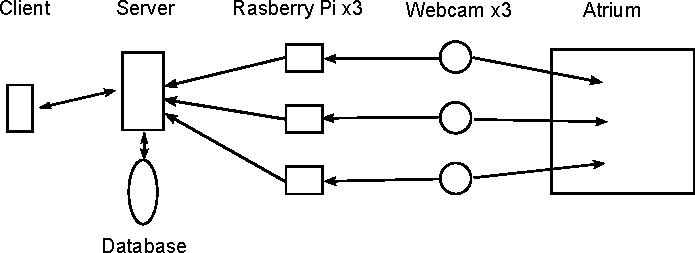
\includegraphics[scale=0.85]{evaluation/evaluation_setup}
	\caption{Experimental Setup}
	\label{fig:evaluation_setup}
\end{figure}

First, three exit areas are manually set in one area by sending requests to the server containing the coordinates of the desired exit points. 

The experiment starts with a single person walking across the monitored areas. We perform a probability request by providing a room id and the id of the detected person, which is stored in the database. The Raspberry Pi sends data about the person's position and room to the server which stores it in the database.

\textit{\textbf{Results.}}
\begin{enumerate}
\item The coordinates of the person are calculated and stored correctly while the id of the object is mistranslated and is stored incorrectly. 
\item The server returns a set of probabilities to each exit, which are not very accurate.
\end{enumerate}

\textit{\textbf{Interpretation.}}
We have found that the outcome of result 1 is due to the server not maintaining a link between each coordinate, thus, the complete path of the person is not stored.
This is crucial since the data about the person's path is essential in calculating probabilities. This is shown in the outcome of result 2 containing inaccurate probabilities. This is because the lack of path information prevents the probability calculations from using the previous position, as well as the entrance area of the occupant. Ultimately, this made us choose to test the prediction model in a separate environment. The tests are described in Section~\ref{eval_prediction}.

\textit{\textbf{Solutions.}} The results in these cases are due to an implementation bug on the server side that was discovered way too late into the project to be fixed. Furthermore, the problem described in the result 2 is the consequence of the result's 1 problem, thus fixing the latter would fix the former one as well.

\section{Scenario 2}
\textit{\textbf{Purpose.}} The purpose of this scenario is to test the image analysis when multiple people are present in the monitored area.

\textit{\textbf{Setup.}} The setup of this experiment is exactly the same as in Scenario~\ref{sec:scen1}.

The experiment starts with multiple people entering and exiting the monitored area.

\textit{\textbf{Results.}}
\begin{enumerate}
\item Several people are moving while keeping a distance of 2 or more meters of each other and are interpreted as separate occupants with different ids.
\item Several people are moving while keeping a distance of less than 2 meters of each other and are interpreted as one occupant with the same id (Figure~\ref{fig:evaluation_1}).
\item Two people are entering the monitored area and are initially interpreted as separate occupants. They intersect and split and are interpreted as new occupants.
\end{enumerate}

\textit{\textbf{Interpretation.}} The outcome of result 2 and 3 is partly due to the camera placement and because the differentiation of the occupants is only based on the positions. 

\textit{\textbf{Solutions.}} In order to handle the problems mentioned in the result 2 and 3, we could possibly change the web camera's position by placing it on the ceiling and facing it down towards the monitored area. In this way, as we have already discussed in the earlier chapters, the camera's field of view would be increased and this would make detection of multiple people walking side by side easier.

However, if we leave the web cameras in the same position, in order to handle the problem, we could possibly change our current approach of detecting people to using human body shape or face recognition techniques. These approaches are more complicated to implement, however they could produce better results when trying to detect, track and differentiation between multiple people walking in the monitored area.

The problem mentioned in the result 3 could possibly be handled by investigating the parameters of the resulting bounding box that was shown in Figure~\ref{fig:evaluation_1}. By finding the average size of a bounding box of one person, we could define a threshold parameter. By comparing the size of person's bounding box with the threshold, we can then have the following situations:

\begin{enumerate}
\item If the resulting bounding box is slightly bigger than the threshold, we can assume that it contains two people. Now, if our assumption turns out to be correct, we can simply go through the list of previously detected people and find two, who are closest to the center of our new bounding box. Finally, to draw two bounding boxes around both occupants, we can examine their shape and try to approximately split them in half. Naturally, this approach is not perfect, as there still be situations of two people being identified as one, if they stand very close to each other, but their bounding box is smaller than the threshold. Furthermore, some people are significantly taller and/or bigger than the average person, thus this algorithm might interpret those people as them being two occupants walking close to each other.
\item In the other situation we might get a bounding box, which is significantly bigger than the threshold. This would possible mean that there are more than two people gathered really closely. Naturally, this situation is even harder to handle, as it is difficult to make a guess on how many people there are in the monitored area, as well as find the previously detected people who were close to this large bounding box.
\end{enumerate}

\begin{figure}[htb]
	\centering
	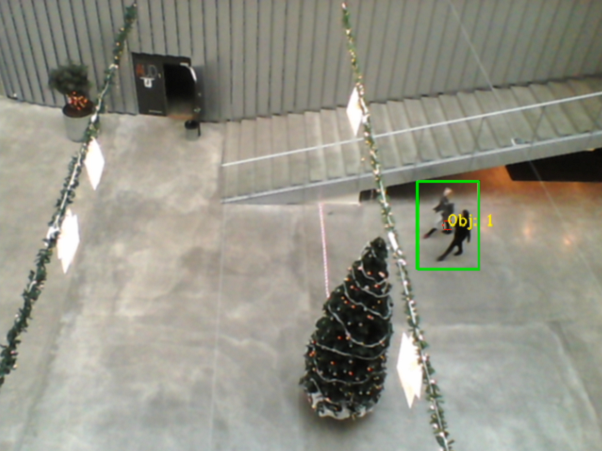
\includegraphics[scale=0.82]{evaluation/evaluation_1}
	\caption{Problem of two people walking too close to each other}
	\label{fig:evaluation_1}
\end{figure}

\section{Prediction model}
\label{eval_prediction}
Due to the issue mentioned in section \ref{sec:scen1}, we continued the testing of the prediction model in a separate program allowing for easy setup of a desired scenario testing various aspects of the prediction model. The program is implemented in C\# and uses the same logic as the Java implementation. Figure \ref{fig:pred_c} shows an image of the program where each cell is marked with the activity value. 

\textit{\textbf{Purpose.}} The purpose of this setup is to test whether the implemented rule sets have an effect.
\begin{figure}[htb]
	\centering
	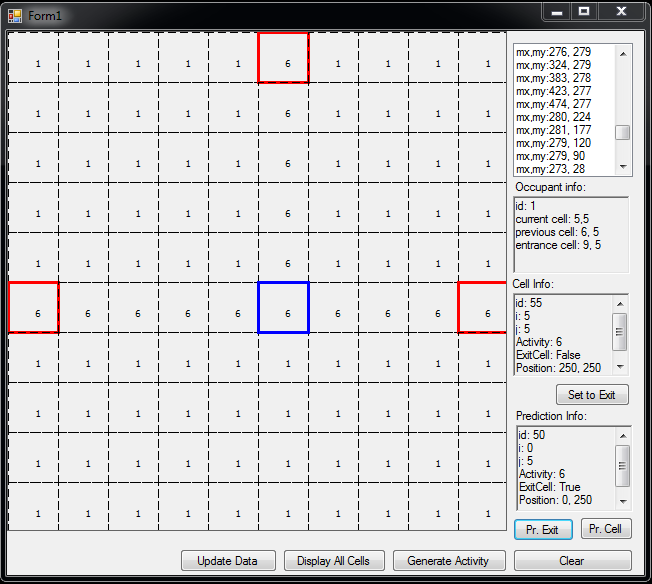
\includegraphics[scale=0.82]{prediction_figures/prediction_csharp}
	\caption{Screenshot of the prediction test program.}
	\label{fig:pred_c}
\end{figure}

\textit{\textbf{Setup.}} The image depicts a scenario where the occupant entered at the right exit and moving left. He is currently positioned at the blue square. By pressing the "Pr. Exit" button the program will perform the calculation. 

\textit{\textbf{Results.}} The left cell is the predicted exit. The probabilities for each exit are only printed to the console in the test program. The results are:
\begin{verbatim}
    Exit at: 0 , 5 , prob=0,3576
    Exit at: 5 , 0 , prob=0,3494
    Exit at: 9 , 5 , prob=0,2930
\end{verbatim}

\textit{\textbf{Interpretation.}} Since each activity value is the same along the paths to each exit, the rules must have had an effect. The occupant is most likely to exit to the left because he came from the right. He is least likely to exit to the right even though he is positioned closer because this exit serves as his entrance. Moving the occupant one cell to the left increases the probability that he will exit to the left to 0,4935. This is intended as the distance to the left exit decreases. Increasing the activity value in the cells along the path to the topmost exit to 7 increase the probability to the topmost exit to 0,3607, making it the predicted exit when the occupant is positioned at the original location.